\subsection{Combining the two radial scales}\label{c4:hierarchical}

We have now proved the three ingredients needed to estimate the two-mark
scalar: its angular-to-radial normalization, the coercivity of its radial
links, and the growth bound for a partially suppressed trace.  We combine
them here.  The larger color block will contribute a factor that cancels
against the Pfaffian denominator; the final estimate depends only on the
shorter arc between the marks.

\begin{theorem}[Uniform two-mark bound]\label{c4:thm-two-mark}
Fix \(C_0\ge1\).  Consider a sequence of the even site arrays defining
\(\mathscr H\) in \eqref{c4:Pair-sum}, with the two allowed shifts of
Section~\ref{c4:pair-confluence}.  Both marked sites have the same shift.
Suppose that
\[
 |L|+1=k\to\infty,\quad 3k\le N\le k^{C_0},\quad N\ {\rm even}.
\]
Here \(L\) denotes the shorter site block; the radial period below will
be denoted \(P\).  Let \(a_i,d_i\) count the unshifted and shifted color
sites, omitting the two marks, in sector \(i\), with sector 1 equal to
\(R\) and sector 2 equal to \(L\).  Assume
\[
 a_1\asymp N,\qquad a_2\asymp k,\qquad a_1\ge a_2,\qquad
 \inf_{0\le\rho\le1}\max_{i=1,2}|d_i/a_i-\rho|\longrightarrow0.
\]
The comparison constants are fixed along the sequence.  Then
\begin{equation}
                         |\mathscr H|\le k^{-4/3+o(1)}.                   \label{c4:H-bound}
\end{equation}
Thus, for every fixed \(\varepsilon>0\), the scalar is at most
\(k^{-4/3+\varepsilon}\) for all sufficiently large members of the
sequence, after absorbing a fixed multiplicative constant into the
exponent loss.
\end{theorem}

\Needspace{5\baselineskip}
\begin{proof}
\leavevmode\par

\paragraph{The profiles and the order of limits.}
Choose angle rays by the spread estimate, from a finite list covering the indicated ratios, so its bounds are uniform. We will bound \(|\mathcal T(P,u_*)|/\mathcal S\), the quantity in \eqref{c4:normalized-two-mark-comparison}. Remove \(b_H\) from the central radial vertex as described after \eqref{c4:PR-d}, extracting the self scale \(\mathcal S\) of \eqref{c4:heavy-self-scale}. Besides unit phases and bounded self constants this factors out image/compensator interactions tending to 1 in the successive limits at each fixed array. Leave deterministic local phases in the links (always unitary scalar factors on each configuration); the oscillator/heat insertions now have bounded charges \(2w,-2v\). The effect from \(b_H\) on roots apart from phases already handled by \eqref{c4:PR-a}--\eqref{c4:PR-c} is by activity multipliers. In sector \(i\) they are 1 identically at \(24,E4\), since all pairings with the heavy orbits vanish. For its strict types \(1F,12,E3\) their pre-periodization logs decay at either infinity as \(O(a_i e^{-|u|/6})\), and modulus of the multiplier at real \(u\) in a base period centered at 0 (also after images) is at most \(\exp(-c a_i e^{-|u|/6})\) by the spread estimate; indeed the logs from each period add. The root phases outside \(0<u<u_*\) and inside are respectively the stationary ones for \(\sigma=0,2v\) with the unit gauge of that calculation (a fixed diagonal conjugation within the segment).

Use width \(D\) fixed sufficiently large. Take the two successive limits along periods \(P=hD\) (even integral \(h\)) and compensator positions \(u_*=j'D\) in boxes far from center and endpoints eventually. As in the preceding comparison we let period tend to infinity first and compensation distance to infinity next. The normalization left to estimate is the radial series times \(\exp(P/32)Z_A^r(P)\) (omitted denominator \(Z_C^r\Theta_C^r\to1\)). Realize it as the trace of links from box \([jD,(j+1)D)\) to the next one, cyclically glued. The states are the same as in the single-mark link construction in Section~\ref{c4:plateau}, now using the present \(A\) for all positive-frequency oscillators and entrance slopes recorded by labels
\[
 s\in\mathcal S_t=1/4+3t/2+\mathbb Z,\qquad t=0,1
\]
outside/inside respectively (before steps at the entrance boundary). Compatibility carries \(s\) forward by adding \(n(b)\) per source-box vertex, including residual marks. The heat momentum is \(m=p\,s/p^2\). The link kernel uses exactly the adjacent-box fractions, mode operator \(e^{a^\dagger(\mathfrak F_j)}\Gamma_{\rm op}(\mathfrak P_D)e^{a(\mathfrak G_{j+1})}\) for interactions beyond the adjacent pairs, and split heat (including telescoping boundary costs) specified in that construction and the adaptation at \eqref{c4:Spread-3}. Replace its per-width prefactor by \(\exp(D/32)\), using source-box local phase and activity rules of \eqref{c4:PR-b},\eqref{c4:PR-c} and self factors, coefficients and measures there. In particular a mark modifies links in which its box is source or target; any constant deterministic phases not assigned to source vertices can just multiply the trace. These links reconstitute the desired trace by the same contraction argument including images and determinant, and are Hilbert--Schmidt uniformly here, Lipschitz in bounded source profiles, by \eqref{c4:Spread-3} and the damping bounds; deterministic phase dependence even on very large \(a_i,d_i\) does not enter the bound.

\paragraph{Three homogeneous operators.}
Define, for each of the two homogeneous slope sectors, operators \(K_t,M_t,J_t\), the unmarked single-link kernel with profiles respectively: all 1; just first-sector strict types zero and others 1; all strict types zero and others 1. Use the stationary phases with \(\sigma_t=2tv\), \(t=0,1\), throughout (or their indicated gauge). These operators are independent of counts. Their powers satisfy:
\par\noindent\textbullet\quad \(K_t\) is power bounded. Indeed \(\operatorname{Tr}K_t^h=Z_C^r(hD)\Theta_C^r(hD)\) at \(h\ge3\) by the stationary identity, so its only possible spectrum near or above modulus 1 is a simple eigenvalue 1.
\par\noindent\textbullet\quad The partially suppressed trace and the link trace have the exact relation
\[
 \operatorname{Tr}(M_t^h)
    = I_{\sigma_t}(hD)Z_C^r(hD)\Theta_C^r(hD),\qquad h\ge3.
\]
The last two factors tend to 1. Hence \eqref{c4:PS-1} and compact
spectral extraction give \(M_t\) spectral radius at most
\(\exp((5/288)D)\).
\par\noindent\textbullet\quad \(J_t\) has as nonzero spectrum, with the free multiplicities,
\[
                \exp\big(D(1/32-s^2/(2p^2)-e)\big),\quad s\in\mathcal S_t,\quad
                e\text{ oscillator excitation for }A .
\]
Indeed \(n(b)=1,2\) respectively for the only active roots \(24,E4\) in each color sector. Traces therefore cannot contain them, using just free \(Z_A^r\), fixed-slope heat and the prefactor. The flag by support on \(s\ge s'\) is invariant, and spectra on the restriction and quotient use the corresponding slope subsets by the same trace calculation. Thus each nonzero eigenvalue's Riesz range is supported at slopes \(\ge\) its minimum displayed label, and its Riesz projector kills inputs supported strictly above its maximum label.

Extraction from traces and norm bounds by regular-radius spectral cuts use exactly the compact-operator argument at \eqref{c4:Link-1}. In particular powers of \(M_t\) are bounded by \(C(\varepsilon)\exp((5/288+\varepsilon)jD)\) at exponent index \(j\ge0\). All constants can be taken uniformly over the finite ray choices.

\paragraph{Decay across the central marked insertion.}
Fix small \(0<\delta<1\), set \(r_i=6\log a_i,\ T=\delta\log k\), and take the successive limits only after making the bounds (period and \(u_*\) arbitrarily large for each \(k,N\)). Put \(m'=\lfloor(r_2-T)/D\rfloor\). In the central \(2m'\) source boxes (indices \(-m',\ldots,m'-1\)), replace strict-root profiles by zero, with error per link smaller than any inverse power by the profile and Lipschitz bounds, including links \(-1,0\) containing the mark. Indeed on these boxes
\(a_i e^{-|u|/6}\ge e^{T/6}=k^{\delta/6}\) for both sectors.
This will also cost only such an error in the trace, as the separate estimates below and the fixed norm bounds across the \(O(\log k)\) core show. The exact core product after replacement is
\[
             J_1^{m'-1} C_N^\circ J_0^{m'-1}
\]
where \(C_N^\circ\) (the two modified links together) is uniformly bounded and increases slope by \(\ge3/2\). Fixed diagonal gauges can equivalently be absorbed into this and the interfacial kernels. Consequently, for any fixed \(\varepsilon>0\),
\[
        \|J_1^{m'-1} C_N^\circ J_0^{m'-1}\|
        \ \le\ C_\varepsilon\exp((-3/16+\varepsilon)(m'-1)D).
\]
To prove this estimate, split the spectra of both \(J_t\) at small regular
radii.  The remainders decay at those radii in operator norm.  Since each
full operator has finite spectral radius, the radii can be chosen so that
any product containing a remainder decays faster than the asserted rate.
There remain finitely many pairs of Riesz subspaces.  The polynomial
factors from possible Jordan blocks can be absorbed into
\(\exp(\varepsilon(m'-1)D)\).

Consider such a retained pair, with sector-0 and sector-1 Riesz
projections \(\mathcal P_{0,L}\) and \(\mathcal P_{1,R}\).
The middle factor in operator order is
\[
             \mathcal P_{1,R}C_N^\circ\mathcal P_{0,L}.
\]
The incoming range of \(\mathcal P_{0,L}\) is supported on slopes at
least its lowest eigenvalue label. The central insertion raises every
slope by at least \(3/2\), and the outgoing projection
\(\mathcal P_{1,R}\) kills inputs supported strictly above its highest
label. Thus the pair vanishes unless there are eigenvalue labels
\(s_L\in\mathcal S_0\), \(s_R\in\mathcal S_1\) with
\(s_R\ge s_L+3/2\).  For those labels,
\[
 s_L^2+s_R^2
   =\tfrac12(s_L+s_R)^2+\tfrac12(s_R-s_L)^2
   \ge\frac98,
 \qquad \frac{s_L^2+s_R^2}{2p^2}\ge\frac14.
\]
The two spectral prefactors contribute \(2/32=1/16\), and oscillator
excitations only decrease the rate.  Hence the paired rate is at most
\(1/16-1/4=-3/16\), proving the estimate.  This is where the joint
two-sided spectral information is used; separate bounds on
\(\|J_0^{m'}\|\) and \(\|J_1^{m'}\|\) would lose the slope jump.

\paragraph{The partially suppressed region and the exterior.}
For source boxes fully within \(r_2+T\le|u|\le r_1-T\) (if nonempty), take period and compensation distance already large enough so there are no marked links there. On either side products then use \(M_t\) plus perturbations whose norms sum to \(O(1)\) uniformly: first-sector strict profiles are super-small and second-sector ones are close to 1 by the complex tail bound including images. Thus these middle products cost at most
\[
                 O_\varepsilon(1)\exp\!\big(2(r_1-r_2)(5/288+\varepsilon)\big)
\]
together, by expanding in perturbations and using the preceding power estimate. Boxes fully exterior to \(r_1+T\) similarly use power-bounded \(K_t\) plus summable perturbations (uniformly bounded norm sum even on the period by exponential image tails). Split at the two compensation links \(j'-1,j'\), keeping their Hilbert--Schmidt product bound for trace norm; homogeneous tail products on each segment cost \(O(1)\). The remaining interface boxes count \(O(1+T/D)\) and cost at most \(\exp(O_D(1+T))\) by fixed bounded-profile norms, even if the two interfaces overlap. These prove also the stated core replacement error by product telescoping since \(r_1=O(\log k)\). In particular the estimates stay bounded in the two successive limits at each fixed large \(k,N\), as needed for removing the heavy-to-image/compensator interactions separately.

The three comparison regions are shown in Figure~\ref{fig:radial-regions}. Their separate bounds now leave only the normalization to be restored.

\begin{figure}[htbp]
\centering
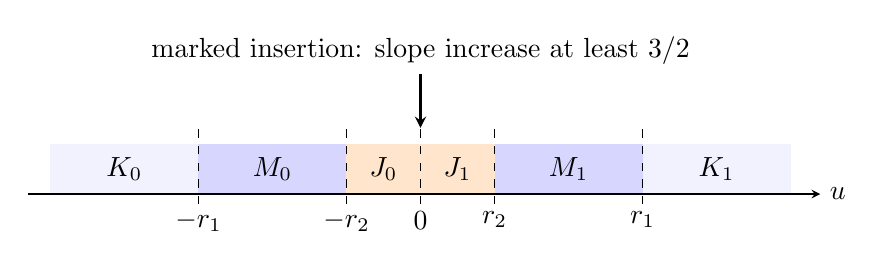
\begin{tikzpicture}[x=.94cm,y=.8cm,>=stealth]
 \fill[blue!5] (-5,0) rectangle (-3,.8);
 \fill[blue!16] (-3,0) rectangle (-1,.8);
 \fill[orange!20] (-1,0) rectangle (1,.8);
 \fill[blue!16] (1,0) rectangle (3,.8);
 \fill[blue!5] (3,0) rectangle (5,.8);
 \draw[->] (-5.3,0)--(5.4,0) node[right] {$u$};
 \foreach \x in {-3,-1,0,1,3} {\draw[dashed] (\x,-.16)--(\x,1.05);}
 \node at (-4,.4) {$K_0$};
 \node at (-2,.4) {$M_0$};
 \node at (-.5,.4) {$J_0$};
 \node at (.5,.4) {$J_1$};
 \node at (2,.4) {$M_1$};
 \node at (4,.4) {$K_1$};
 \node[below] at (-3,-.12) {$-r_1$};
 \node[below] at (-1,-.12) {$-r_2$};
 \node[below] at (0,-.12) {$0$};
 \node[below] at (1,-.12) {$r_2$};
 \node[below] at (3,-.12) {$r_1$};
 \draw[->,thick] (0,1.9)--(0,1.05);
 \node[above,align=center] at (0,1.9) {marked insertion: slope increase at least $3/2$};
\end{tikzpicture}
\caption{The two radial scales, with $r_i=6\log a_i$ and $a_1\ge a_2$.
The central region suppresses both sets of strict roots and is compared
with $J_t$. The next region suppresses only the first set and is compared
with $M_t$; the exterior is compared with $K_t$. The transitions have
width $O(\delta\log k)$ in the proof. The diagram is schematic and does
not depict the exceptional case in which the middle intervals disappear.}
\label{fig:radial-regions}
\end{figure}


\paragraph{Cancellation of the larger scale.}
Each side of the central insertion has length
\((m'-1)D=6\log k-T+O(1)\).
The paired decay is therefore \(k^{-9/8+O(\delta)+O(\varepsilon)}\).
The two intermediate regions have combined length at most
\(12\log(a_1/a_2)+O(T+D)\).  Their rate \(5/288\) contributes
\((a_1/a_2)^{5/24}\).  Since \(a_1\asymp N\) and
\(a_2\asymp k\), all the estimates together give
\[
 \limsup_{u_*\to\infty}\limsup_{P\to\infty}
      \frac{|\mathcal T(P,u_*)|}{\mathcal S}
 \le k^{-9/8}(N/k)^{5/24}\ k^{O_D(\delta)+O_{C_0}(\varepsilon)+o(1)}.
\]
Fixed multiplicative constants are absorbed into the exponent loss.
Equation~\eqref{c4:normalized-two-mark-comparison} now restores the lattice normalization at a cost
\(N^{-5/24+o(1)}\).  Its dependence on the total size cancels:
\[
 k^{-9/8}(N/k)^{5/24}N^{-5/24}=k^{-4/3}.
\]
The condition \(N\le k^{C_0}\) converts all residual \(o(1)\) powers of
\(N\) into \(o(1)\) powers of \(k\).  We first keep \(D\) fixed, then
let \(\delta,\varepsilon\) decrease to zero.  This proves
\eqref{c4:H-bound}, with the stated uniform exponent slack.
\end{proof}
